\section{Análise Discriminante}

	``A análise discriminante é uma \textbf{técnica multivariada} que \textbf{cria funções discriminantes}, provenientes de combinações lineares das variáveis iniciais, que maximizam as diferenças entre as médias dos grupos e minimizam a probabilidade de classificações incorretas dos casos nos grupos.

	É aplicada quando a \textbf{variável dependente é qualitativa} (grupos) e as \textbf{variáveis independentes são quantitativas}. As variáveis dicotômicas, como sexo, podem também ser incluídas nas variáveis explicativas.

	A análise discriminante \textbf{tem por objetivo escolher as variáveis que distinguem os grupos}, de modo que, conhecendo-se as características de um novo caso, se possa prever a que grupo pertence.

	A análise discriminante pode ser usada também para validar a análise de cluster e confirmar os resultados da análise fatorial". \cite{torres}

	\subsection{Hipóteses}

		$
			\begin{cases}

				\mathsf{H}_{0} : & \text{Não há diferença. As variáveis não discriminam os objetos investigados} \\
				\mathsf{H}_{a} : & \text{Há diferença. As variáveis discriminam os objetos investigados}

			\end{cases}
		$

		\bigskip

		\textbf{Observações}

			Se as variáveis têm uma diferença de grandeza entre elas, será preciso então padronizá-las para que a análise discriminante não as discrimine por essa razão.

	\subsection{Pressupostos}

		\subsubsection{Cada grupo é uma amostra aleatória de uma população normal multivariada}

			``A sua violação pode levar a decisões incorretas, principalmente quando as amostras são pequenas. \textbf{Quando a violação da normalidade se deve apenas à não simetria da distribuição, a potência do teste não é afetada}, contrariamente ao que acontece se a \textbf{distribuição não for mesocúrtica} e, de forma mais acentuada, se for platicúrtica, caso em que devemos optar pela regressão logística". \cite{torres}

			Para medir a curtose, divida a "estatística" pelo "erro padrão" (SPSS). Para verificar se ela é mesocúrtica, veja se o valor fica entre $-1,96 < x > +1,96$ . (Padronização Z: $1,96 = 0,475$ $\rightarrow$ 95\% no total (bicaudal)).

			Verifique os outliers. A remoção de outliers pode aproximar as variáveis para a normal. Outliers moderados não costumam criar grande impacto nas análises.

		\subsubsection{Dentro dos grupos a variabilidade é idêntica, isto é, as matrizes de variância e covariância são iguais para todos os grupos}

			Teste homocedasticidade, equivalente multivariado ao teste de Levene.

			``A verificação deste pressuposto é feita na própria análise discriminante, através do \textbf{teste Box’s M}. Caso seja violado, aumenta a probabilidade dos casos serem classificados no grupo com maior dispersão.

			A violação deste pressuposto afeta a análise principalmente quando os grupos não têm igual dimensão, mesmo que as diferenças sejam moderadas" \cite{torres}.

			\bigskip

			\textbf{Dicas e Recomendações \cite{torres}}

				\begin{itemize}
					\item O número mínimo de observações por variável independente: 5 ;
					\item Número recomendado de observações por variável: 20 ;
					\item Número de observações por grupo: o menor grupo deve ter um tamanho que exceda o número de variáveis independentes;
					\item É recomendável que o número mínimo de casos em cada grupo seja 20, e que os grupos tenham dimensões semelhantes.
				\end{itemize}
				
	\subsection{Análise Discriminante no SPSS \cite{torres}}

		\subsubsection{Teste M de Box(\textit{Box's M})}

			``Este teste verifica um dos pressupostos na análise discriminante (\textbf{pressuposto da homocedasticidade}). Ele testa se as diferentes dispersões são ou não estatisticamente significativas. É muito sensível a afastamentos da normalidade".

			O teste Box's M é muito ``sensível à desvios de normalidade e à dimensão das amostras (amostras grandes conduzem geralmente à rejeição de Ho)". Para solucionar uma possível violação do pressuposto da homocedasticidade  é importante ter uma amostra grande com o mesmo número de observações em cada grupo. ``Segundo alguns autores, a análise discriminante é uma técnica bastante robusta à violação dos pressupostos, desde que a \textbf{dimensão do menor grupo seja superior ao número de variáveis independentes em estudo}".

			\bigskip

			\textbf{Hipóteses}

				\bigskip

				$
					\begin{cases}

					\mathsf{H}_{0} : & \text{As matrizes observadas de variância-covariância são iguais entre grupos} \\
					\mathsf{H}_{a} : & \text{As matrizes observadas de variância-covariância não são iguais entre grupos}

					\end{cases}
				$

			\bigskip \bigskip

			\textbf{Tabela}

				\begin{figure}[H]
					\centering
					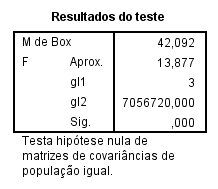
\includegraphics[height=5.5cm]{images/analise-discriminante_teste-box-s-m}
				\end{figure}
				
		\subsubsection{Teste Lambda de Wilks (\textit{Wilk's Lambda})}

			``O Wilk’s Lambda dá informação sobre as diferenças entre os grupos, para cada variável individualmente. Obtém-se pela razão entre a variação dentro dos grupos e a variação total.

			Este teste é robusto a violação do Teste Box’s M quando os grupos têm dimensões semelhantes.

			A não rejeição da hipótese de igualdade da média de uma variável nos grupos ($\alpha > 0,05$), aumenta a probabilidade de ser classificada incorretamente em outro grupo".

			\bigskip

			\textbf{Tabela de Estatísticas de Grupo}

				Será que essas médias são significativamente diferentes (pela variabilidade das mesmas) ou elas podem ser consideradas iguais?

				\begin{figure}[H]
					\centering
					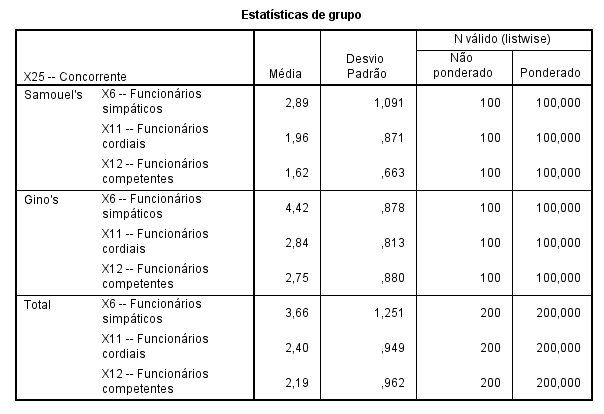
\includegraphics[height=10cm]{images/analise-discriminante_estatisticas-de-grupo}
				\end{figure}

			\textbf{Hipóteses}

				\bigskip

				$
					\begin{cases}

					\mathsf{H}_{0} : & \text{Não existe diferença entre as médias dos grupos} \\
					\mathsf{H}_{a} : & \text{Existe diferença entre as médias dos grupos}

					\end{cases}
				$

			\bigskip \bigskip

			\textbf{Tabela Lambda de Wilks}

				\begin{figure}[H]
					\centering
					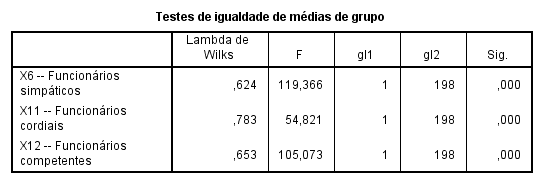
\includegraphics[height=5cm]{images/analise-discriminante_lambda-de-wilks}
				\end{figure}

				``Neste caso, como temos 3 variáveis, devemos comparar a significância com $\alpha / 3 = 0,05/3 = 0,017 $ e não com $\alpha = 0,05$. Como todas as significâncias são $< 0,017$, devemos rejeitar $\mathsf{H}_{0}$.

				A tabela mostra que existe diferenças significativas nas médias de cada variável nos dois grupos ($\text{significâncias} = 0,000$), não informando, entretanto, sua importância para discriminar grupos".

		\subsubsection{Contribuição das Variáveis}

			\paragraph{Matrizes intragupos em pool \textit{Pooled within-groups matrices}} \hspace{0cm}

				``Na sua interpretação tem de se levar em consideração a correlação entre as variáveis explicativas, pois se duas variáveis tiverem correlação $1$, incluir ambas não fornece mais informação do que incluir uma só. Por isso o uso da opção \textit{Stepwise}".

				\begin{figure}[H]
					\centering
					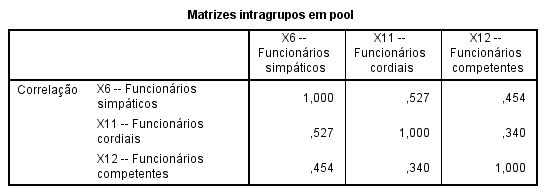
\includegraphics[height=5.5cm]{images/analise-discriminante_matrizes-intragupos-em-pool}
				\end{figure}

				Nessa tabela, "como podemos observar, não existe problema de \textbf{multicolinearidade}, uma vez que nenhum coeficiente de correlação entre variáveis independentes é superior, em termos absolutos, a $0,9$.

				Quando há multicolinearidade, não se deve analisar a importância de cada variável para a análise, visto que sua elevada correlação com outras a torna redundante. Nesta situação apenas se usa o procedimento \textit{Stepwise}".
				
			\paragraph{Estatísticas \textit{Stepwise}} \hspace{0cm}

				\begin{figure}[H]
					\centering
					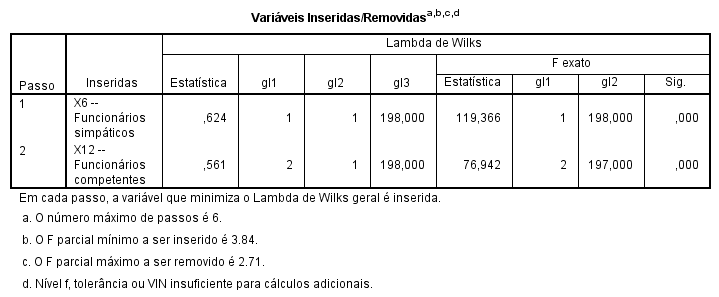
\includegraphics[height=6.5cm]{images/analise-discriminante_stepwise_var-inseridas-removidas}
				\end{figure}

				$
					\begin{cases}

					\mathsf{H}_{0} : & \text{A separação dos grupos não foi bem sucedida (em função das médias)} \\
					\mathsf{H}_{a} : & \text{A separação dos grupos foi bem sucedida (em função das médias)}

					\end{cases}
				$

				\bigskip \bigskip

				``A tabela acima resume o procedimento Stepwise, indicando para cada passo que variáveis foram adicionadas/removidas, o valor de Wilk’s Lambda e a significância. Note que a cada passo, a variável “escolhida” é aquela que minimize o valor de Wilk’s Lambda, isto é, aquela para a qual ocorrem maiores diferenças entre as médias dos grupos, até que não ocorram variação significativas de Lambda.

				O Teste Wilk’s Lambda avalia se o modelo consegue separar e classificar bem os grupos.

				Neste caso, com uma significância menor que $0,05$, podemos dizer que a separação dos grupos foi bem sucedida".

				\begin{figure}[H]
					\centering
					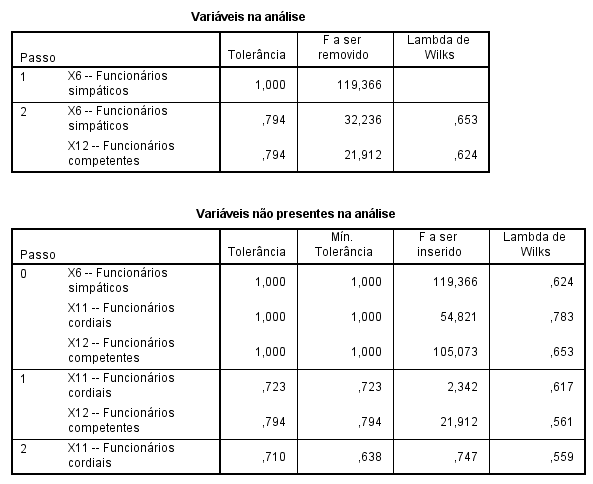
\includegraphics[height=13cm]{images/analise-discriminante_stepwise_var-presentes-e-n-presentes}
				\end{figure}

				``O quadro acima apresenta, para cada passo, as variáveis que foram consideradas como discriminantes na análise. Essas variáveis foram escolhidas como as “melhores”, com base na matriz de correlação, seu poder de discriminação entre grupos e cálculo da tolerância (avaliação da multicolinearidade. Valores muito baixos demonstrariam multicolinearidade).

			\paragraph{Sumarização de funções discriminantes canônicas} \hspace{0cm}

				\begin{figure}[H]
					\centering
					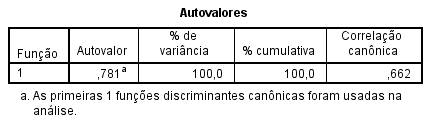
\includegraphics[height=3.5cm]{images/analise-discriminante_sumarizacao_autovalores}
				\end{figure}

				``A tabela acima indica que a variância (em termos da diferença entre os grupos) é explicada em 100\% pela função discriminante".

				\begin{figure}[H]
					\centering
					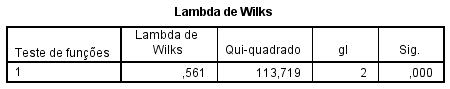
\includegraphics[height=2.5cm]{images/analise-discriminante_sumarizacao_lambda-de-wilks}
				\end{figure}

				$
					\begin{cases}

					\mathsf{H}_{0} : & \text{A função discriminante não é significativa} \\
					\mathsf{H}_{a} : & \text{A função discriminante é significativa}

					\end{cases}
				$

				\bigskip

				Neste caso ``a função discriminante é significativa para separar os grupos".

				\begin{figure}[H]
					\centering
					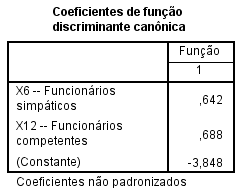
\includegraphics[height=6cm]{images/analise-discriminante_sumarizacao_coeficiente-de-funcao-d-c-}
				\end{figure}

				A tabela acima é "usada para escrever a(s) função(ões) discriminante(s)".

				\bigskip

				{\Large Função $= -3,848 + (0,642 * \mathsf{X}6) + (0,688 * \mathsf{X}12)$}

				\bigskip

				Considere $\mathsf{X}6 = 2$ e  $\mathsf{X}12 = 1$ $\rightarrow$ Função $= -1,8768$ $\rightarrow$ Pertence ao Samouel's (Olhe a tabela do centróide mais abaixo)

				\bigskip

				Considere $\mathsf{X}6 = 4$ e  $\mathsf{X}12 = 3$ $\rightarrow$ Função $= 0,7818$ $\rightarrow$ Pertence ao Gino's (Olhe a tabela do centróide mais abaixo)
				
			\paragraph{Estatísticas de classificação} \hspace{0cm}

				\begin{figure}[H]
					\centering
					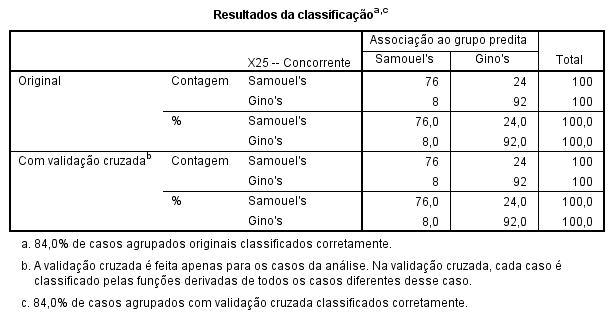
\includegraphics[height=8cm]{images/analise-discriminante_classificacao_resultados}
				\end{figure}

				``Finalmente, a tabela acima apresenta os resultados da classificação. Repare que 76\% dos clientes do Samouel's foram classificados corretamente e que 24\% dos clientes foram classificados como clientes do Ginos's. Além disso, 92\% dos clientes do Gino's foram classificados corretamente e 8\% não".

				\begin{figure}[H]
					\centering
					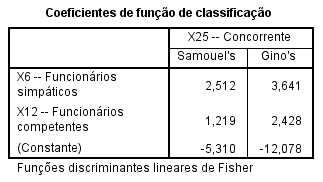
\includegraphics[height=5cm]{images/analise-discriminante_classificacao_coeficientes-de-funcao}
				\end{figure}

				A tabela acima é utilizada para escrever a(s) função(ões) para alocação dos dados.

				\bigskip

				{\Large Função Samouel's $= -5,310 + (2,512 * \mathsf{X}6) + (1,219 * \mathsf{X}12)$}

				\bigskip

				{\Large Função Gino's $= -12,078 + (3,641 * \mathsf{X}6) + (2,428 * \mathsf{X}12)$}

				\bigskip

				Condidere $\mathsf{X}6 = 2$ e  $\mathsf{X}12 = 1$

				\bigskip

				Função Samouel's $= -5,310 + (2,512 * 2) + (1,219 * 1) = 0,933$
				
				Função Gino's $= -12,078 + (3,641 * 2) + (2,428 * 1) = -2,368$

				\bigskip

				Condidere $\mathsf{X}6 = 4$ e  $\mathsf{X}12 = 3$

				\bigskip

				Função Samouel's $= -5,310 + (2,512 * 4) + (1,219 * 3) = 8,359$
				
				Função Gino's $= -12,078 + (3,641 * 4) + (2,428 * 3) = 9,77$

				\begin{figure}[H]
					\centering
					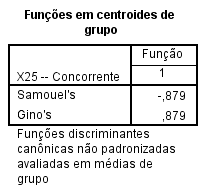
\includegraphics[height=6.5cm]{images/analise-discriminante_centroides-de-grupo}
				\end{figure}

				``Uma abordagem final para exame de diferenças entre grupos é o centróide. Em uma análise discriminante com dois grupos temos dois centróides, com três grupos três centróides, etc.

				Os centróides para nosso exemplo mostra que o do Samouel’s é $-0,879$ e do Gino’s $0,879$. Esta é uma medida de síntese global que indica que o Gino’s é percebido de maneira muito mais positiva do que o Samuel’s".

		\subsubsection{Passo a Passo}

			Não esqueça de verificar os pressupostos da análise antes de fazê-la.

			\begin{figure}[H]
				\centering
				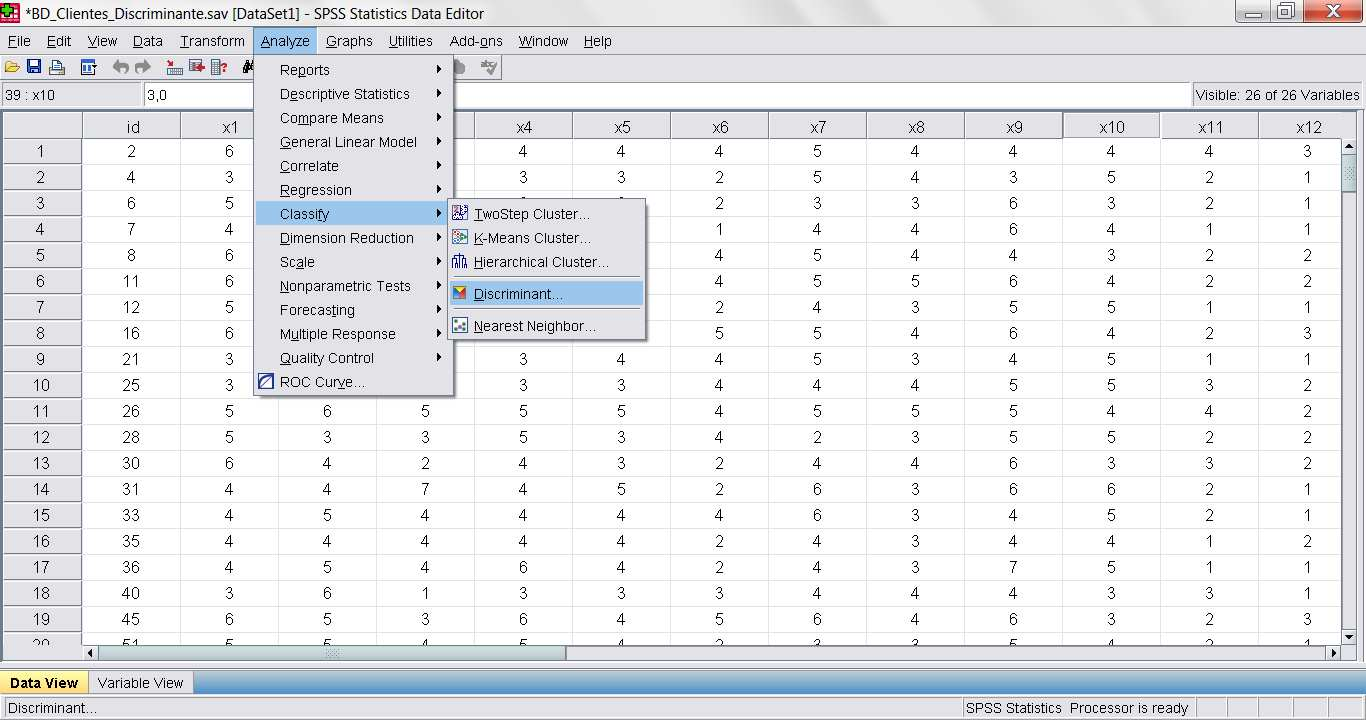
\includegraphics[height=8cm]{images/analise-discriminante_passo-a-passo_1}
			\end{figure}			
			
			\begin{figure}[H]
				\centering
				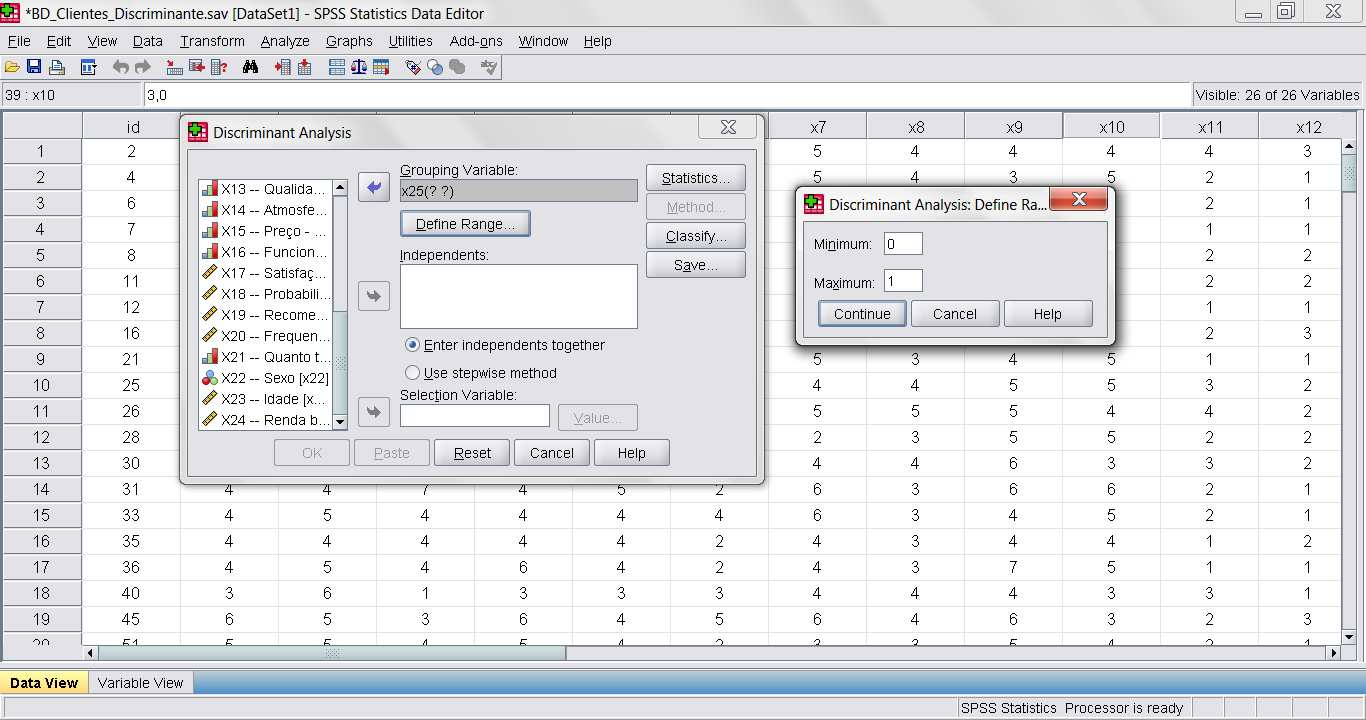
\includegraphics[height=8cm]{images/analise-discriminante_passo-a-passo_2}
			\end{figure}
			
			\begin{figure}[H]
				\centering
				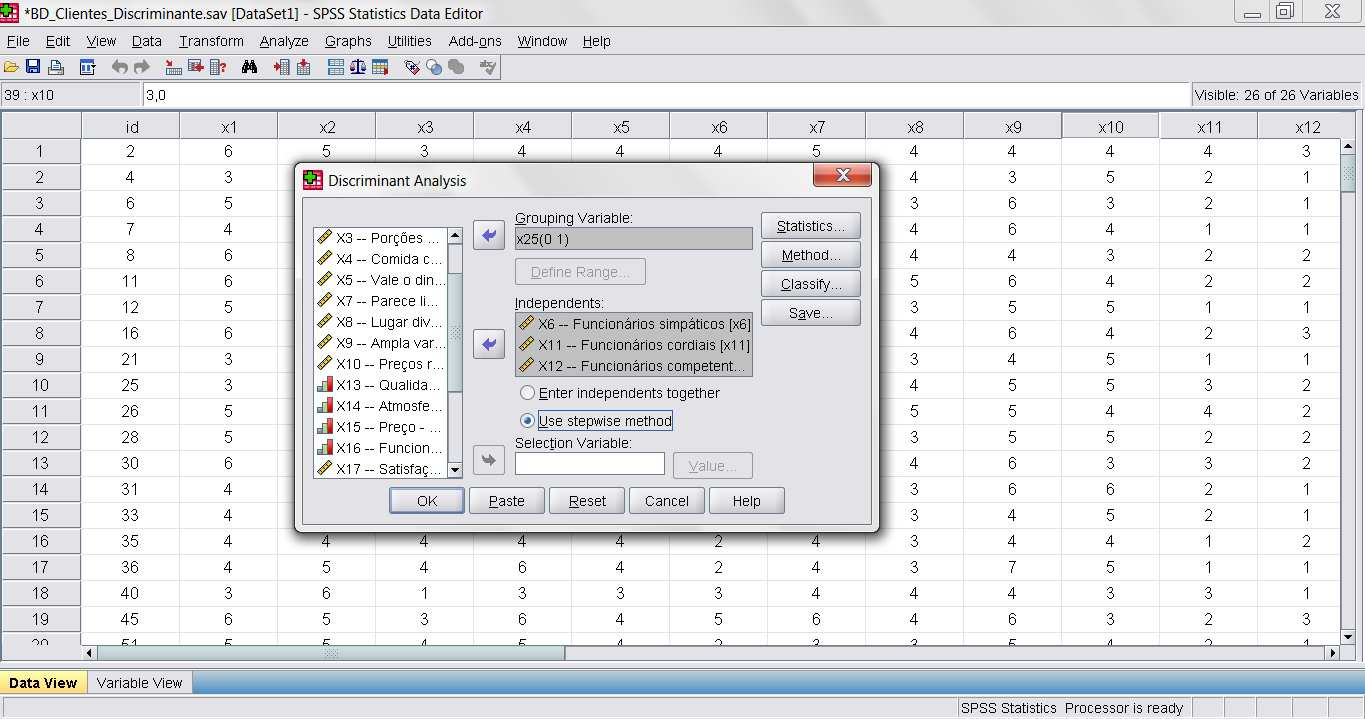
\includegraphics[height=8cm]{images/analise-discriminante_passo-a-passo_3}
			\end{figure}

			\begin{figure}[H]
				\centering
				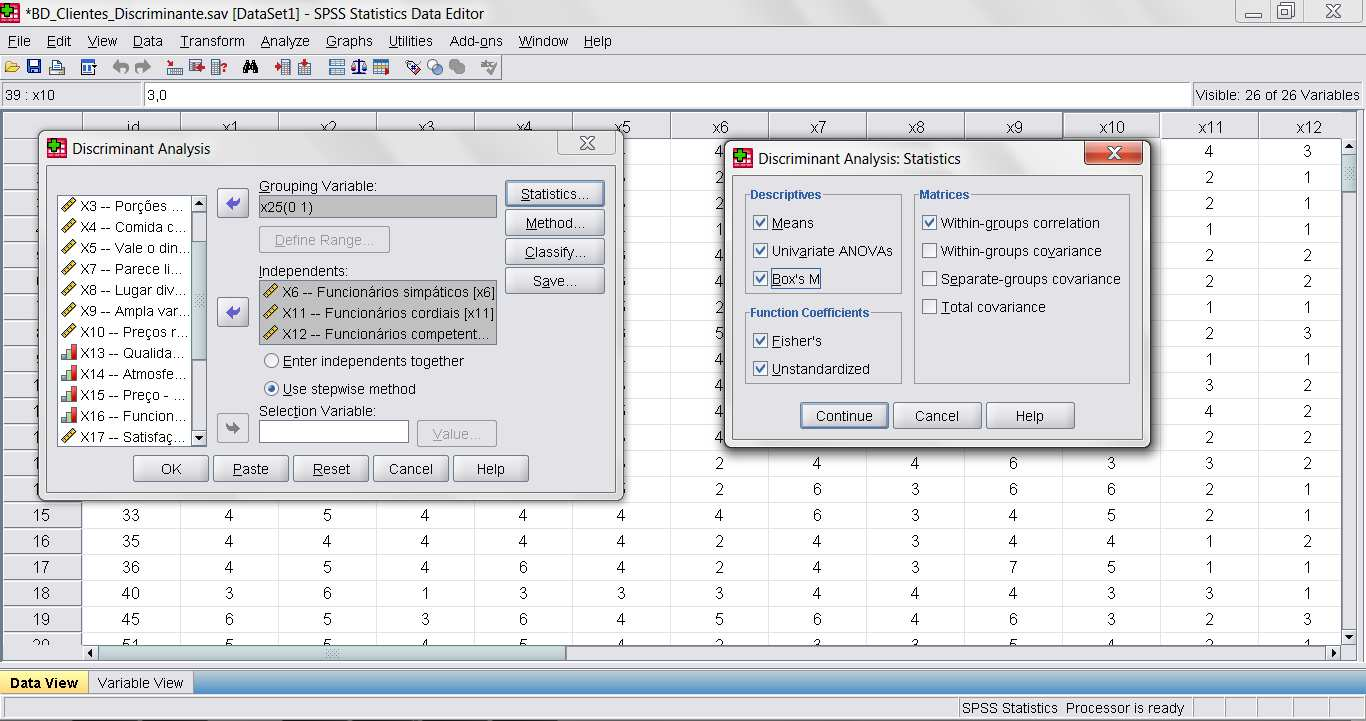
\includegraphics[height=8cm]{images/analise-discriminante_passo-a-passo_4}
			\end{figure}

			\begin{figure}[H]
				\centering
				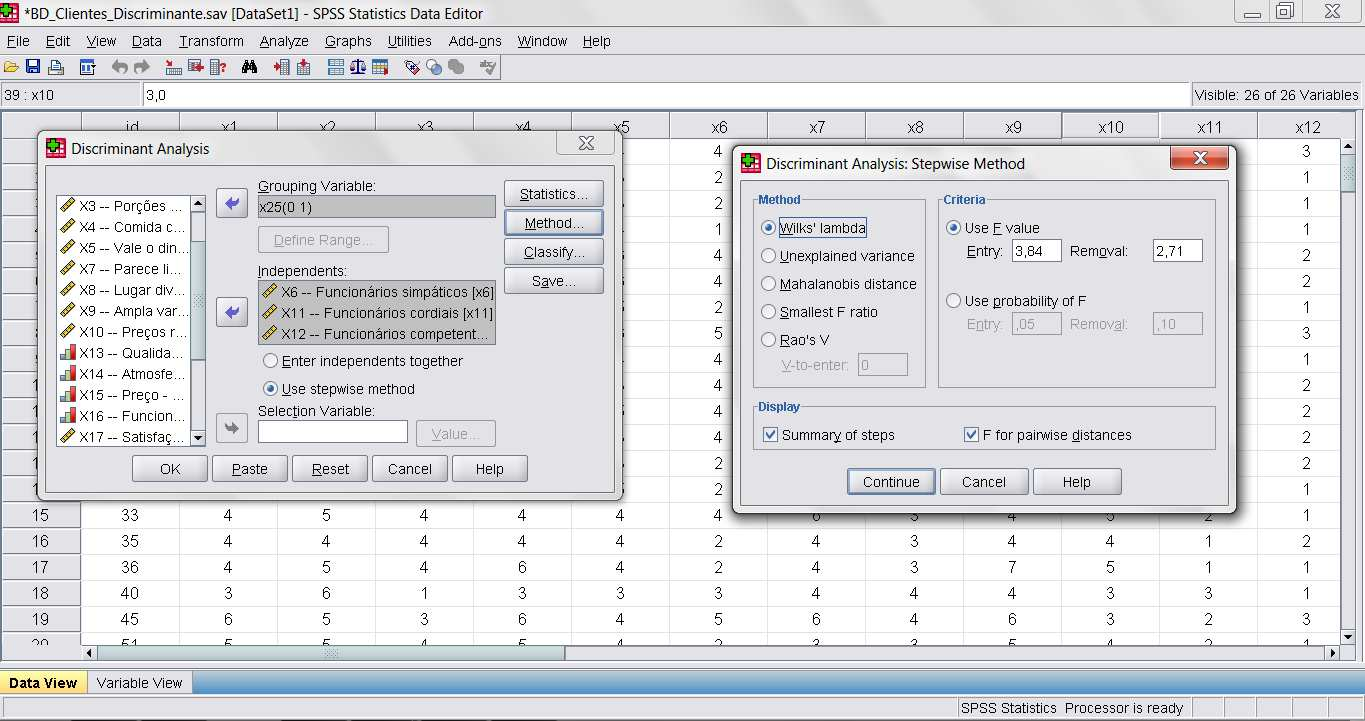
\includegraphics[height=8cm]{images/analise-discriminante_passo-a-passo_5}
			\end{figure}

			\begin{figure}[H]
				\centering
				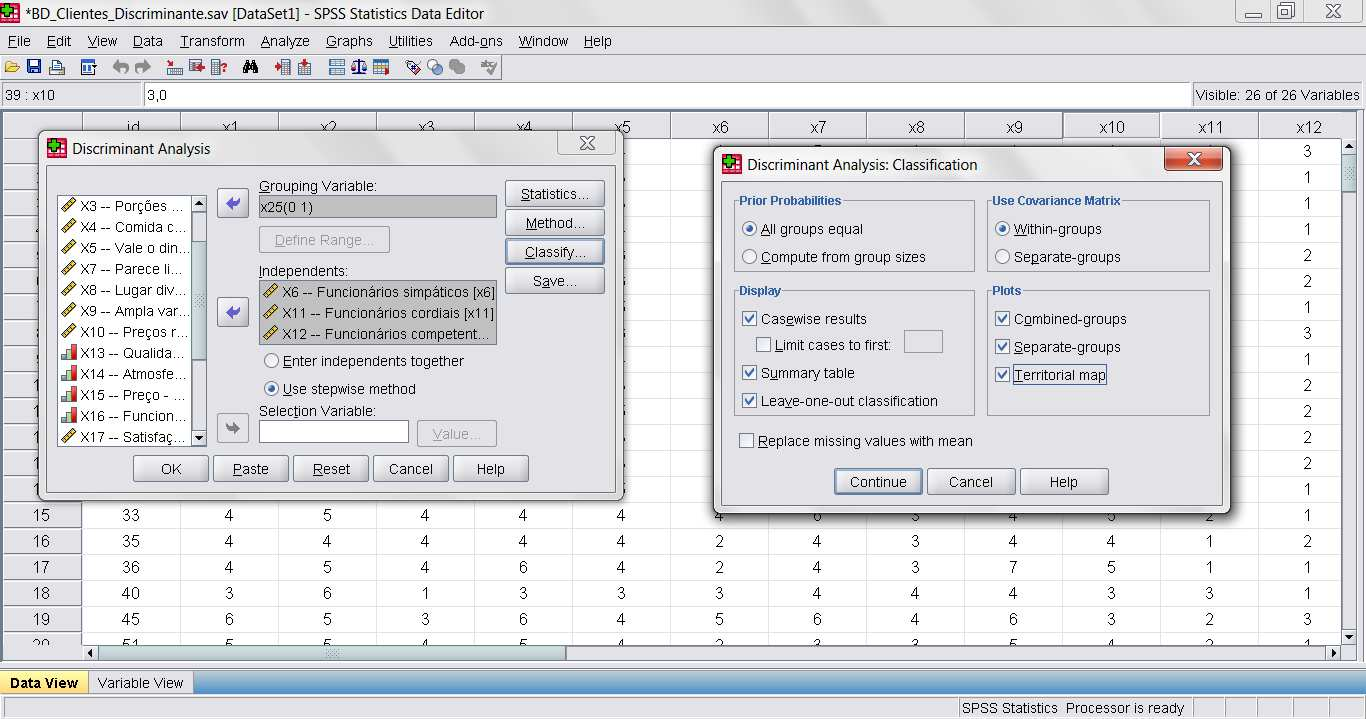
\includegraphics[height=8cm]{images/analise-discriminante_passo-a-passo_6}
			\end{figure}

			\begin{figure}[H]
				\centering
				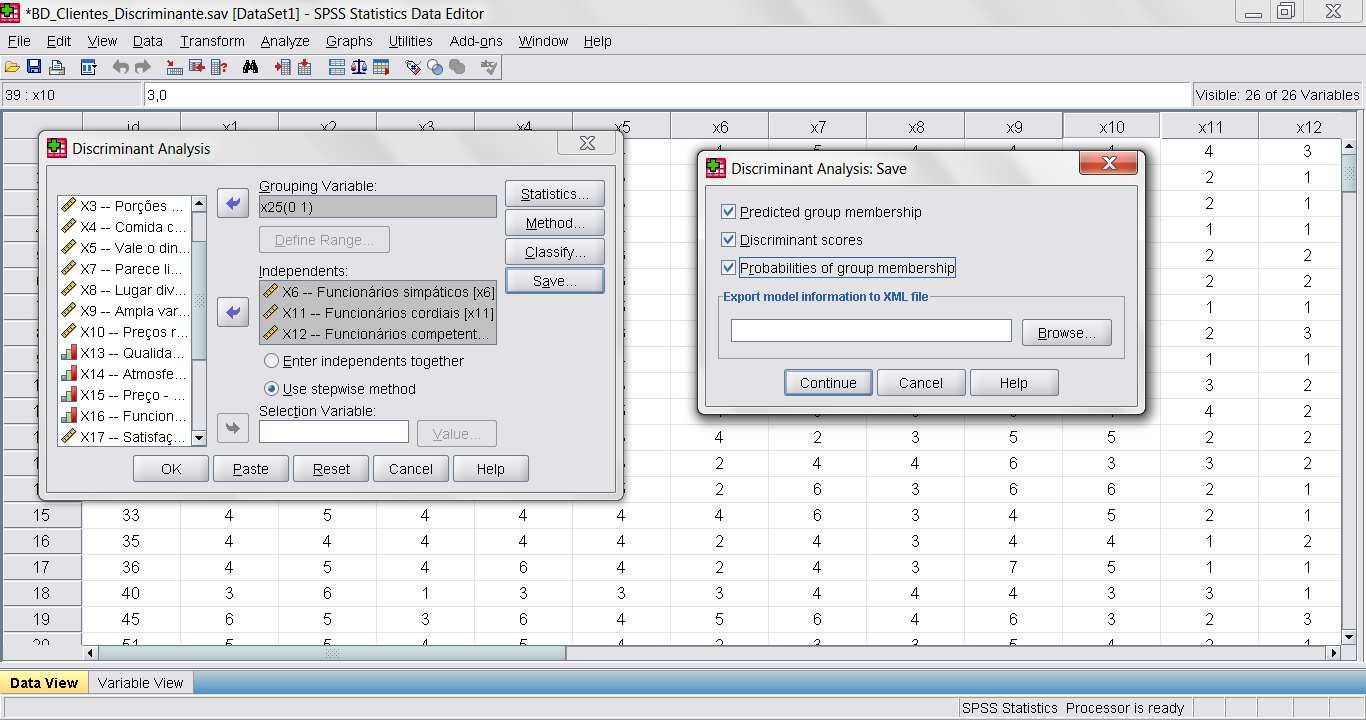
\includegraphics[height=8cm]{images/analise-discriminante_passo-a-passo_7}
			\end{figure}